\chapter{Geophysical Seismic Imaging} 

\section{Introduction} 
The Earth is characterised by seismic activities. Human has been always animated by the curiosity to understand these activities. During years, human used different techniques to explore the basement depths. Recently, this exploration is more motivated by multiples reasons that can be economics, social, environment, scientific etc. For instance, the study of the nature the soil is useful for civil engineers, landslide imaging is very useful for estimating the risk of gravity, the detection of oil and mineral resources present a major economic challenge, the monitoring of radioactive waste landfill areas or CO2 injection represents an new environmental challenge.  

With the advents of Industrial revolution accompanied by the higher need to find new oilfield by hydrocarbon industry, the \textit{seismic imaging} technique has successfully used from the mid of 19th. By definition, seismic imaging is a tool that bounces sound waves off underground rock structures to reveal the possible tectonic structures \cite{Reddy2012}. In seismic modelling, one need data coming from seismic wave propagation to create good quality images of the subsurface (imaged by acoustic waves). The acoustic waves are generated under the Earth by sources that can be man-made devices or by earthquakes. Receivers or seismometers acquire information that can provide details of the velocity and the geometric structure of the Earth \cite{Reddy2012}. 


During years scientists invent several techniques of seismic imaging which include \textit{Electrical Resistivity Tomography},  \textit{Ground penetrating radar}, \textit{Induced polarization}, \textit{Seismic Tomography} and \textit{Reflection seismology} \cite{Reddy2012}.

\subsection{Electrical Resistivity Tomography (ERT)} The ERT technique is invented by Schlumberger brothers and developed by the work of Andrey Nikolayevich Tikhonov . This method is an electrical testing method where electrical current is induced in the ground between one pair of electrodes and the voltage is measured between another pair. These measurements are used to estimate lateral and vertical variations of resistivity values of the earth. ERT can be used to map geologic variations (soil lithology, presence of ground water, fracture zones, variations in soil saturation, areas of increased salinity or, in some cases, ground water contamination), bedrock depths and geometry, mapping cavities such as caves, karst and/or evaporate dissolution sinkholes. Like other seismic technique, ERT has the capacity to yield either 1D (sounding), 2D (profile) or 3D (volume) imaging.  

\subsection{Ground Penetrating Radar (GPR)} GPR systems work by sending a tiny pulse of energy into a material via an antenna. An integrated computer records the strength and time required for the return of any reflected signals. Subsurface variations will create reflections that are picked up by the system and stored on digital media. This technique has many applications: civil engineering, resources explorations.  

\subsection{Induced Polarization (IP)} Similar to electrical resistivity tomography, this technique measure the electrical chargeability of subsurface materials. IP provide additional information about the spatial variation in lithology and grain-surface chemistry. It can be made in time-domain and in frequency-domain.  IP method is widely used in mineral exploration and mining industry and it has other applications in hydrogeophysical surveys, environmental investigations and geotechnical engineering projects.
 
\subsection{Reflection Seismology (RF)} This is the most wide used technique when we talk about hydrocarbon exploration, or mineral exploration. RF is a form of echo sounding, detecting echoes from seismic interfaces. It can yield results that are the closest of any geophysical technique to a conventional geological section. The waves propagation under the Earth require to know some features of the wave: transmission, absorption, and attenuation in the earth materials and its reflection, refraction, and diffraction characteristics
at discontinuities.   

In the context of onshore, geophysicists use geophones as receivers to collect the speeds of particles on the ground. Accelerometer sensors can be used to record these data. These sensors are directional and measure the speed or acceleration in a spatial direction. Sometimes, devices with multi-components are used to measure wavefields in the horizontal directions (parallel to the Earth's surface) and vertical direction, thus identifying the different types of waves whose depend on the directions \cite{BROSSIERPhD}. The figure \ref{geophones} shows the scenario of data acquisition with geophones.  

\begin{figure}[!h]
% Use "\centering" in floats (figure, table), but if you need to center
% some text (why?) use "\begin{center}...\end{center}".
\centering 
% Figure environments same as 0.8 * \textwidth please
% That does not necessarily mean the actual picture size,
% it is a guideline for the environment which could contain
% 2 or more pictures! Be consistent and follow the guidelines
% provided in your sources.
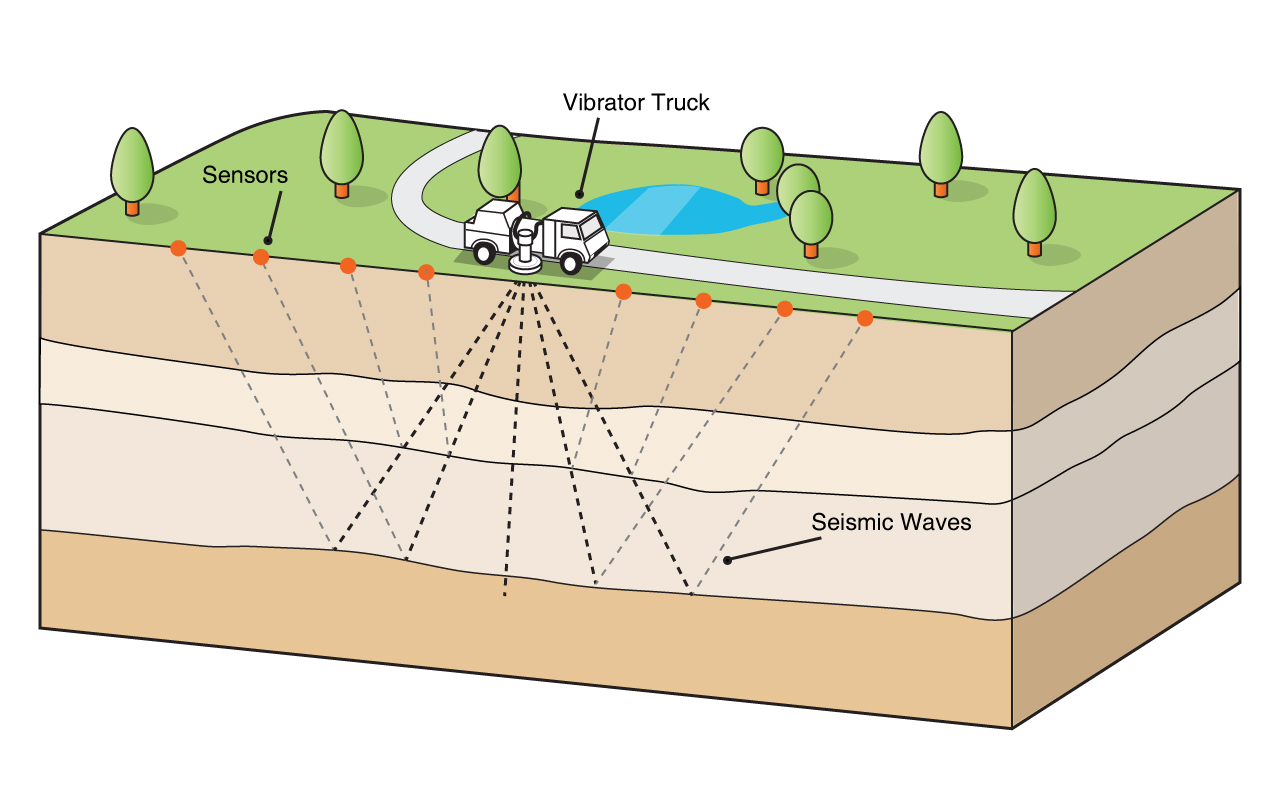
\includegraphics[width=0.6\textwidth]{images/geophones.jpg}
\caption{Seismic imaging}
\label{geophones} 
% if you move the label it breaks the reference numbering; 
% always have it *after* the caption.
\end{figure}

In the off-shoring scenario, the hydrophones, placed on the surface of the sea, are often used to collect the seismic wavefields information. In the figure \ref{hydrophones}, a ship generates the seismic source by an air gun and drag behind, under the water surface, a raw of hydrophones measuring the pressure field which indicates the waves propagated in the structure of the subsoil. Others sensors named \textit{Ocean Bottom Seismometer} (OBS) are designed to record the earth motion under oceans and lakes from man-made sources. These devices can stay several days under the water. Each OBS receives different acoustic waves for each generation of sound arriving at different times. There exists another device called Ocean Bottom Cable (OBC).The data acquisition is performed by multi-component sensors bound on the cables \cite{BROSSIERPhD}. 
\begin{figure}[!h]
% Use "\centering" in floats (figure, table), but if you need to center
% some text (why?) use "\begin{center}...\end{center}".
\centering 
% Figure environments same as 0.8 * \textwidth please
% That does not necessarily mean the actual picture size,
% it is a guideline for the environment which could contain
% 2 or more pictures! Be consistent and follow the guidelines
% provided in your sources.
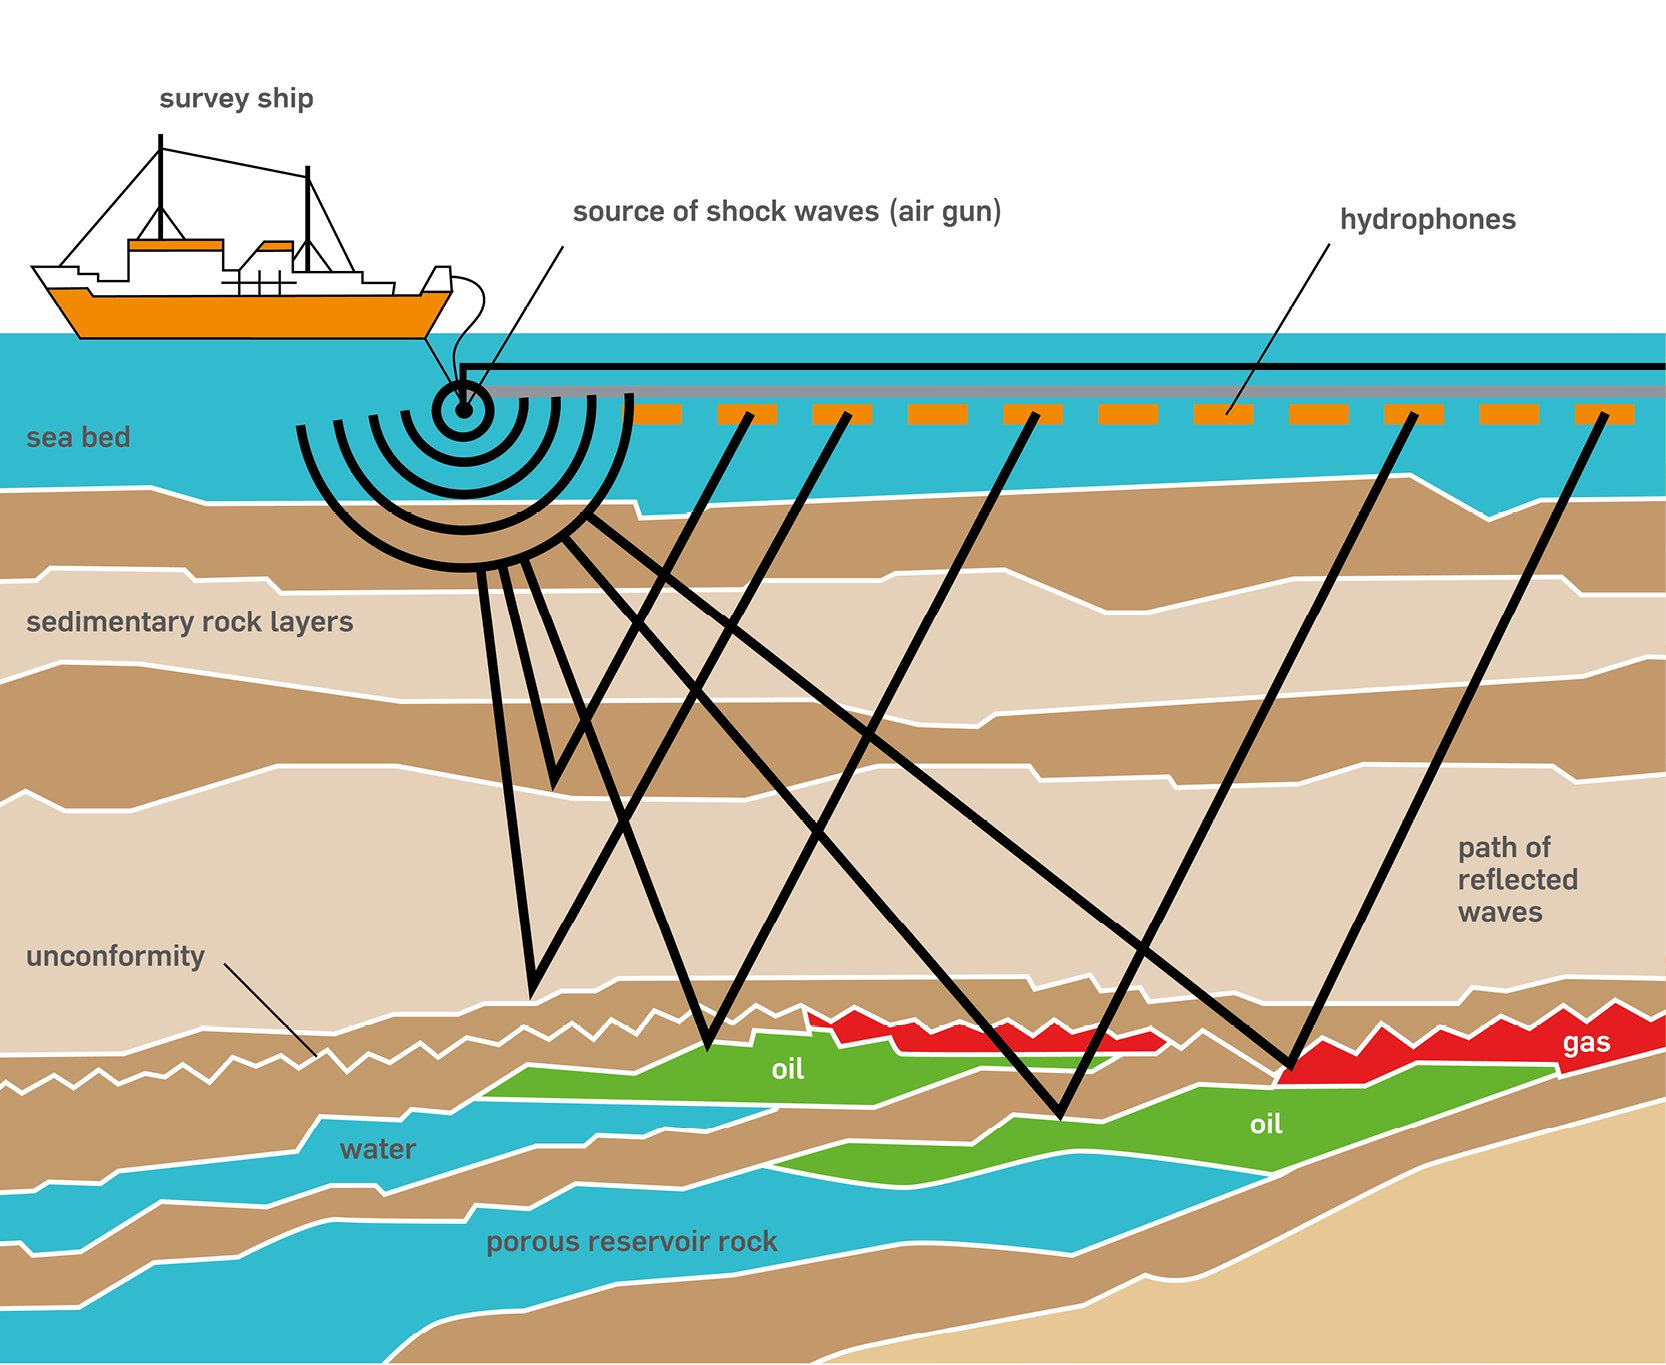
\includegraphics[width=0.6\textwidth]{images/hydrophones.jpg}
\caption{Seismic imaging}
\label{hydrophones} 
% if you move the label it breaks the reference numbering; 
% always have it *after* the caption.
\end{figure}


\section{Seismic model}
These techniques need numerical methods to solve the seismic imaging problem. In this study, we just focus on Frequency-domain seismic modelling based on the sparse direct solver (DSFDM) and Full Wave Inversion (FWI) method used by Seiscope Consortium to develop the DSFDM/FWI code.

The DSFDM is a finite-difference frequency-domain method, which has aimed to solve linear systems resulting from the discretization of the time-harmonic wave equation with sparse direct solvers. This method with 27 stencils has developed in a visco-accoustic \textit{vertical transverse isotropic} (VTI) \cite{Operto2007, Operto2015, Amestoy2016, Brossier2010, Brossier2014}. It is governed by the linear systems resulting by 3D visco-acoustic VTI wave equation:
\begin{align}
Ap_h &= b   \label{eq1}\\
p_v &= Bp_h + s^{'}, \label{eq2}\\
p &= (2p_h + p_v)/3 \label{eq3}
\end{align}
where the matrices $ A $ and $ B $ result from the discretization of operators.

\begin{align}
A &= \omega^{2} \left[ \frac{\omega^{2}}{\kappa_{0}} + (1+2 \epsilon) (\mathcal{X} + \mathcal{Y}) + \sqrt{1+2\delta} \mathcal{Z} \frac{1}{\sqrt{1+2\delta}} \right] \label{eq4}\\
B &= \frac{1}{\sqrt{1+2\delta}} + \frac{2(\epsilon - \delta)\kappa_{0}}{\omega^{2}\sqrt{1+2\delta}} (\mathcal{X} + \mathcal{Y}) 
\end{align}

Similarly, the source terms are given by:

\begin{align}
b &= \frac{\omega^{4}s_{h}}{\kappa_{0}} s - \omega^{2}\sqrt{1+2\delta} \mathcal{Z} \left(s_{v} - \frac{1}{\sqrt{1+2\delta}}s_{h} \right)s, \label{eqb}\\
s^{'} &=  \left(s_{v} - \frac{1}{\sqrt{1+2\delta}}s_{h} \right)s
\end{align}

The wavefields $ p_h = \sigma_{xx} = \sigma_{yy} $ and $ p_v = \sigma_{zz} $ are the so-called horizontal and vertical pressure wavefields, respectively \cite{Plessix2011}. The angular frequency is denoted by $ \omega$, $ \kappa_{0} = \rho V_{0}^{2} $  where $ \rho $ is the density and $ V_0 $ is the vertical wavespeed, $ \delta $ and $ \epsilon $ are the Thomsen's parameters. The seismic source vector is compactly denoted by $ s $. For an explosion and vertical force, the expression of the source vector is given by 
\begin{align}
s_{explosion} &= s(\omega) \hat{\delta}(x_s - x) \\
s_{vertical_force} &= s(\omega)d_z \hat{\delta}(x_s - x) 
\end{align}

where $s(\omega)$ denotes the Fourier coefficient of the temporal source wavelet for the modeled frequency, $d_z$ the derivative with respect to $z$,$\hat{\delta}$ the delta function, $x_s$ the coordinates of the source position. 

The $s_h$ and the $s_v$terms are given by the following formulas.
\begin{align}
s_h &= (2(2+\epsilon)+ \sqrt{1+2\delta})/D, \\
s_v &= (1+2\sqrt{1+2\delta})/D, \\
D &=  4\sqrt{1+2\epsilon} + 4 \sqrt{1+2\delta} + 1
\end{align}
The expression of $ D $ was corrected relative to the one provided in Operto et al. (2014). \newline
The second-order differential operators $  \mathcal{X}$ , $ \mathcal{Y}$ and $ \mathcal{Z}$ are given by
$$ \mathcal{X} = \partial_{\tilde{x}} b  \partial_{\tilde{x}},  \mathcal{Y} = \partial_{\tilde{y}} b  \partial_{\tilde{y}},  \mathcal{Z} = \partial_{\tilde{z}} b  \partial_{\tilde{z}},  $$

where $b=1/\rho$ is the buoyancy and the complex-valued coordinate system $(\tilde{x}, \tilde{y}, \tilde{z})$ is used to implement perfectly-matched layers absorbing boundary conditions \cite{Operto2007}.
If we assume that $\delta$ is slowly varying and hence can be considered as locally homogeneous, the operator $ A $ can be simplified as
\begin{equation}
A_{a} = \omega^{2} \left[ \frac{\omega^{2}}{\kappa_{0}} + (1+2 \epsilon) (\mathcal{X} + \mathcal{Y}) + \mathcal{Z} \right] 2 \mathcal{Z}\kappa_{0} (\epsilon - \delta)  (\mathcal{X} + \mathcal{Y}) \label{eq13}
\end{equation}
In this case, the wave operator within the bracket describes wave propagation in an elliptic medium,
while the second term accounts for anellipticity.

In \textit{elliptic} media $ (\delta=\epsilon \neq 0 ) $, the source become

\begin{align}
b &= \frac{\omega^{4} s_h}{\kappa_{0}} s \\
s^{'} &= 0
\end{align}

The authors mention  this point because the second term of the source $b$, equation \ref{eqb}, involves a second-order vertical derivative which can be tricky to implement if the source does not match the grid point. Therefore, it is worth assuming that the medium is elliptic at the source positions if this is a reasonable assumption.

In isotropic media $(\delta = \epsilon = 0)$, one can easily check that Equations \ref{eq1}-\ref{eq3} reduces to
\begin{equation}
\left[ \frac{\omega^{2}}{\kappa} \mathcal{X} + \mathcal{Y} + \mathcal{Z} \right] p=\frac{\omega^{2}}{\kappa} s \label{eq16}
\end{equation}

where the operator $\left[ \frac{\omega^{2}}{\kappa} \mathcal{X} + \mathcal{Y} + \mathcal{Z} \right]$ represents the operator $A_{iso}$

Similarly, the operator $A$ can be rewritten considering the NMO velocity $(V_{NMO} = V_0\sqrt{1+2\delta} )$ in the diagonal term. This introduces the $\eta = \frac{\epsilon -\delta}{1+2\delta}$ parameter in the coefficients of the matrix.
\begin{equation}
A_{NMO} = \omega^{2} \left[ \frac{\omega^{2}}{\kappa_{NMO}} + (1+2 \eta) (\mathcal{X} + \mathcal{Y}) + \sqrt{1+2\delta} \mathcal{Z} \frac{1}{\sqrt{1+2\delta}} \right]+ 2 \sqrt{1+2\delta} \mathcal{Z} \frac{\kappa_{NMO}}{\sqrt{1+2\delta}} (\mathcal{X} + \mathcal{Y})\label{eq17}
\end{equation}
\textbf{Algorithm.} \newline
The system of three equations \ref{eq1}-\ref{eq3} is solved with the following sequence.
\begin{itemize}
\item Solve the linear system, equation \ref{eq1}, for $p_h$ with a sparse direct solver.
\item Compute explicitly $p_v$ from $p_h$, equation \ref{eq2}.
\item Compute explicitly $p$ from $p_h$ and $p_v$, equation \ref{eq3}.
\end{itemize}
The computational cost of the last two steps is negligible relative to that of the first step.

Note that wave-equation operators \ref{eq4}, \ref{eq13}, \ref{eq16} and \ref{eq17} are implemented in DSFDM code. (See Documentation)

\section{Full Wave Inversion (FWI)}
The Full Wave Inversion is a non linear-data fitting method that enable to get detailed estimates of subsurface properties from seismic data, which can be the result of either passive or active seismic experiments. Basically, initialising a guess of the subsurface parameters (a model), the data are predicted from the solution of the wave propagation equation. And then, the model is always updated to minimize the misfit function between the observed and predicted data. The figure \ref{FWI} illustrates the FWI procedure. \eqref{eq1}

\begin{figure}[!h]
% Use "\centering" in floats (figure, table), but if you need to center
% some text (why?) use "\begin{center}...\end{center}".
\centering 
% Figure environments same as 0.8 * \textwidth please
% That does not necessarily mean the actual picture size,
% it is a guideline for the environment which could contain
% 2 or more pictures! Be consistent and follow the guidelines
% provided in your sources.
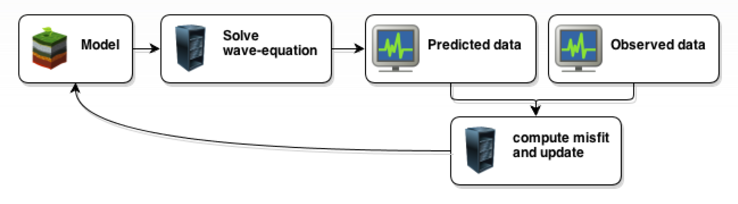
\includegraphics[width=0.8\textwidth]{images/FFWI.png}
\caption{Full Wave Inversion (FWI) procedure. from []}
\label{FWI} 
% if you move the label it breaks the reference numbering; 
% always have it *after* the caption.
\end{figure}

Mathematically, the FFWI can be formulated as an optimization problem. In \cite{Virieux2009}, Virieux and Operto give the main theoretical aspects of FWI based on a least-squares local optimization approach. In a data-domain frequency-domain, FWI is an iterative reduction of the misfit function C defined as the least-squares norm of the difference between recorded and modelled monochromatic pressure data, $ d_{obs} $ and $ d(m)$, respectively.

$$ \min_{m} C(m) = \min_{m} \sum_{\omega} \Vert d_{obs} - d(m) \Vert $$

The subsurface model updated at iteration $ k + 1 $ is given by:

$$ m_{k+1} = m_{k} - \gamma_{k} \mathbf{H}_{k} \nabla_{m} C_{k} $$

where $ \mathbf{H}_{k} \nabla_{m} C_{k} $,the direction of gradient is given by the product of the gradient of C by an approximation of the inverse Hessian, H. The step length $ \gamma_{k} $ defines  quantity of descent. The descent direction can be preconditioned by a diagonal approximation of the Hessian, in our case, the diagonal elements of the so-called pseudo-Hessian matrix \cite{Shin2001}, the aim of which is to balance the gradient amplitudes with respect to depth by removing geometrical spreading effects. 

The expression of the gradient preconditioner is given by:
\begin{equation}
H = 1/ [P + \epsilon max(P)],
\end{equation}
where $P = diag \Re \left\lbrace (\frac{\partial A}{\partial m}p_h)^{\dagger}, (\frac{\partial A}{\partial m}p_h)\right\rbrace, \frac{\partial A}{\partial m}p_h$ are the so-called virtual sources  \cite{Pratt1998} and the
damping factor $\epsilon$ should be chosen with care to balance properly in depth the gradient without generating
instabilities. For more details about full-waveform inversion see \cite{Virieux2009}.

The FFWI code is implemented with SEISCOPE optimization toolbox which contains different optimization algorithms (steepest-descent, conjugate gradient, l-BFGS, truncated Newton) including the line search (see documentation).

\section{Application: Valhall}
The Seismic imaging was applied in Vallhal dataset with Full Waveform Inversion method in the context of SEISCOPE project \cite{Operto2014, Operto2015, Amestoy2016}.
\begin{figure}[!h]
% Use "\centering" in floats (figure, table), but if you need to center
% some text (why?) use "\begin{center}...\end{center}".
\centering 
% Figure environments same as 0.8 * \textwidth please
% That does not necessarily mean the actual picture size,
% it is a guideline for the environment which could contain
% 2 or more pictures! Be consistent and follow the guidelines
% provided in your sources.
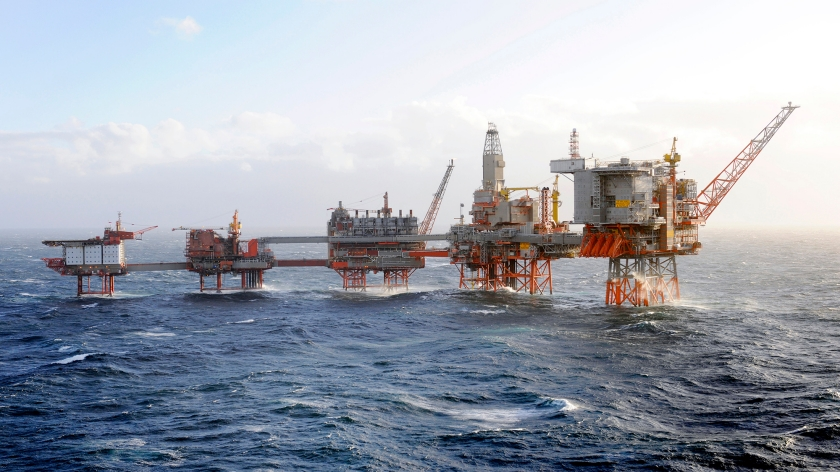
\includegraphics[width=0.6\textwidth]{images/valhall.jpg}
\caption{Valhall offshore}
\label{valhall} 
% if you move the label it breaks the reference numbering; 
% always have it *after* the caption.
\end{figure}
The Valhall oil field is an offshore field located in North Sea in 70 m of water (see figure \ref{valhall}). In this oilfield, the presence of gas cloud is observed in the overburden. The reservoir is approximatively located in 2.5 km depth \cite{Barkved2010}. The data acquisition was making possible by wide aperture/azimuth acquisition covering a surface of 145 $km^{2}$. A layer of 12 cables contains 2302 hydrophones, which record 49,954 explosive sources located 5 m below the surface of the water (Figure \ref{sim1}.a). A distance of 300 m separate two cables except two outer cables at 600 m. 
\begin{figure}[!h]
% Use "\centering" in floats (figure, table), but if you need to center
% some text (why?) use "\begin{center}...\end{center}".
\centering 
% Figure environments same as 0.8 * \textwidth please
% That does not necessarily mean the actual picture size,
% it is a guideline for the environment which could contain
% 2 or more pictures! Be consistent and follow the guidelines
% provided in your sources.
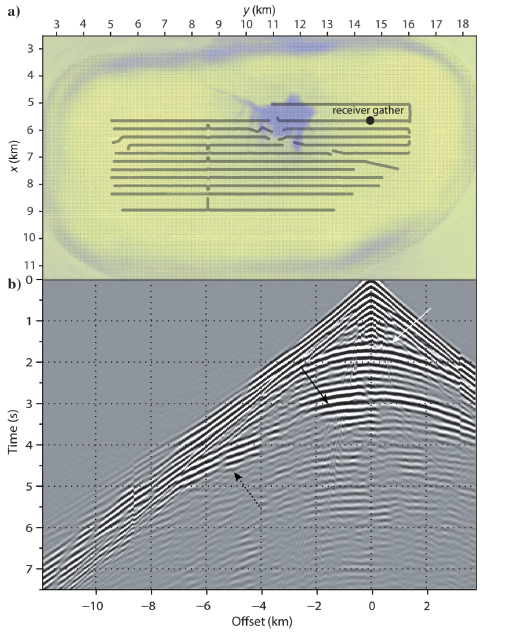
\includegraphics[width=0.6\textwidth]{images/sim1.png}
\caption{ North Sea case study. (a) Acquisition layout and Valhall model  \cite{Amestoy2016}}
\label{sim1} 
% if you move the label it breaks the reference numbering; 
% always have it *after* the caption.
\end{figure}
The figure \ref{sim1}.a shows the gas cloud intersecting the cables (area covered by the 50,000 explosive sources) and the receiver position, whose records are shown in panel. In figure \ref{sim1}.b, the solid black arrow indicate precritical reflection from the reservoir, the dashed black arrow points to the critical and postcritical reflection, and the white arrow points to the reflection from the top of the gas \cite{Operto2015, Amestoy2016}.

In the study of \cite{Operto2015}, a case study of valhall data set shows approximately the presence of gas at 2.5km in depth []. With initial condition $V_0$, vertical-velocity, $\epsilon$ and $\delta$,  Thomsen's parameters, and the density $\rho = -0.0261 V^{2}_{0} + 0.373 V_0 + 1.458$ are used to apply frequency-domain FWI on the OBC data set \cite{Operto2015, Amestoy2016}. With discrete frequencies chosen in the 3.5-10 Hz frequency band, the DSFDM/FWI code was performed in computer nodes that are equipped with two 2.5 GHz Intel Xeon IvyBridge E5-2670v2 processors with 10 cores per processor. the shared memory per node is 64 GB. The connecting network is InfiniBand fourth data rate (FDR) at 56 Gb/s. The operations are performed in single-precision complex arithmetic, for which the peak performance of the machine is 10 Gflops/s/core (which corresponds to a double precision peak of 20 Gflops/s/core) \cite{Operto2015}. Figures \ref{sim2} \ref{sim3} show the 2D and 3D visualisations in different levels of the reservoir of the gas cloud.
According to the authors, this study reveals memory consumption in the step of LU factorisation. They showed that the complexity can reach $O (n^{6}) $ \cite{Operto2015}.
%\begin{figure}[!h]
%% Use "\centering" in floats (figure, table), but if you need to center
%% some text (why?) use "\begin{center}...\end{center}".
%\centering 
%\begin{minipage}{0.6\textwidth}
%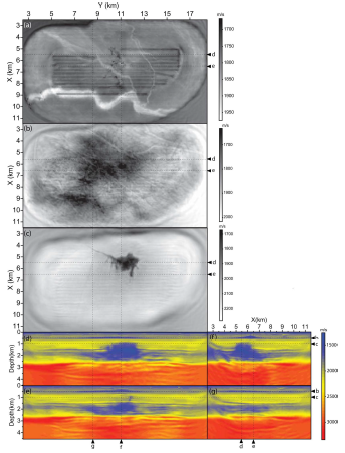
\includegraphics[width=0.6\textwidth]{images/sim2.png}
%\label{sim2} 
%\end{minipage}
%\hfill
%\begin{minipage}{0.6\textwidth}
%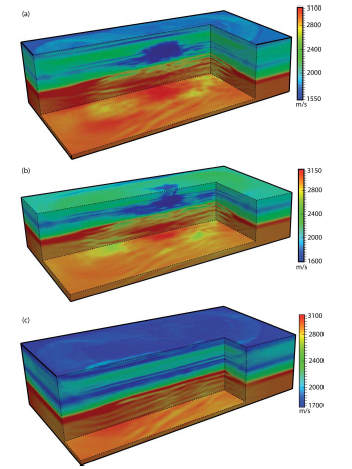
\includegraphics[width=0.6\textwidth]{images/3Dsim3.png}
%
%\label{sim3} 
%\end{minipage}
%\caption{Full Wave Inversion (FWI) procedure. from []}
%\end{figure}

\begin{figure}
\centering 
  \begin{subfigure}[b]{0.4\textwidth}
    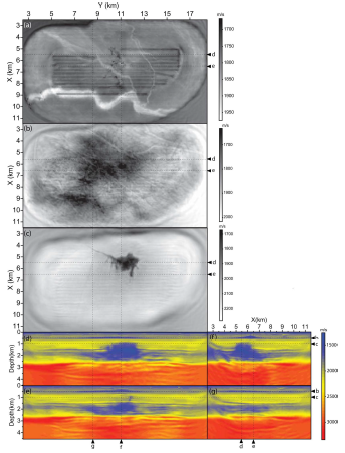
\includegraphics[width=\textwidth]{images/sim2.png}
    \caption{Slices of the 10Hz FWI model, that can be compared with those of the initial model\cite{Operto2015}. }
    \label{sim2}
  \end{subfigure}
  %
  \begin{subfigure}[b]{0.4\textwidth}
    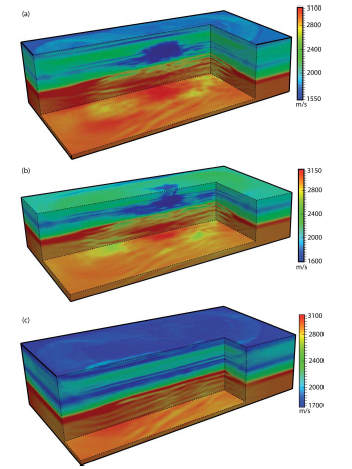
\includegraphics[width=\textwidth]{images/3Dsim3.png}
    \caption{3-D perspectives of the final FWI model.}
    \label{sim3}
  \end{subfigure}
  \caption{Seismic imaging of Valhall \cite{Operto2015}}
\end{figure}
%\section{Challenges of HPC in the context of 3D Seismic Imaging}

This application shows how high performance computing (HPC) is important in the geophysical seismic modelling. Because of the complexity of the problem, one can't think to compute seismic imaging in classical machines. The HPC technology has developed in parallel to improve the performance of problems with high complexity.